\documentclass[tikz,border=8pt]{standalone}
% Shared look for every TikZ diagram. Load with \input{../../tools/tikz-style.tex}
\usepackage[T1]{fontenc}
\usepackage{lmodern}
\renewcommand{\sfdefault}{lmr}  % diagrams use the same serif as the text
\usetikzlibrary{arrows.meta, positioning, shapes.geometric, calc, fit, backgrounds}
\definecolor{cblue}{HTML}{4C78A8}
\definecolor{corange}{HTML}{F58518}
\definecolor{cgreen}{HTML}{54A24B}
\definecolor{cred}{HTML}{E45756}
\definecolor{cpurple}{HTML}{B279A2}
\definecolor{cgrey}{HTML}{6B6B6B}
\tikzset{
  every picture/.style={font=\sffamily, line width=1.2pt},
  box/.style={draw=#1, fill=#1!12, rounded corners=4pt, align=center, inner sep=7pt, minimum height=1.1cm},
  box/.default=cgrey,
  arrow/.style={-{Stealth[length=3mm]}, draw=cgrey, line width=1.4pt},
  title/.style={font=\sffamily\bfseries\Large},
  note/.style={font=\sffamily\small, text=cgrey, align=center},
}
\AtBeginDocument{\hyphenpenalty=10000 \exhyphenpenalty=10000}

\begin{document}
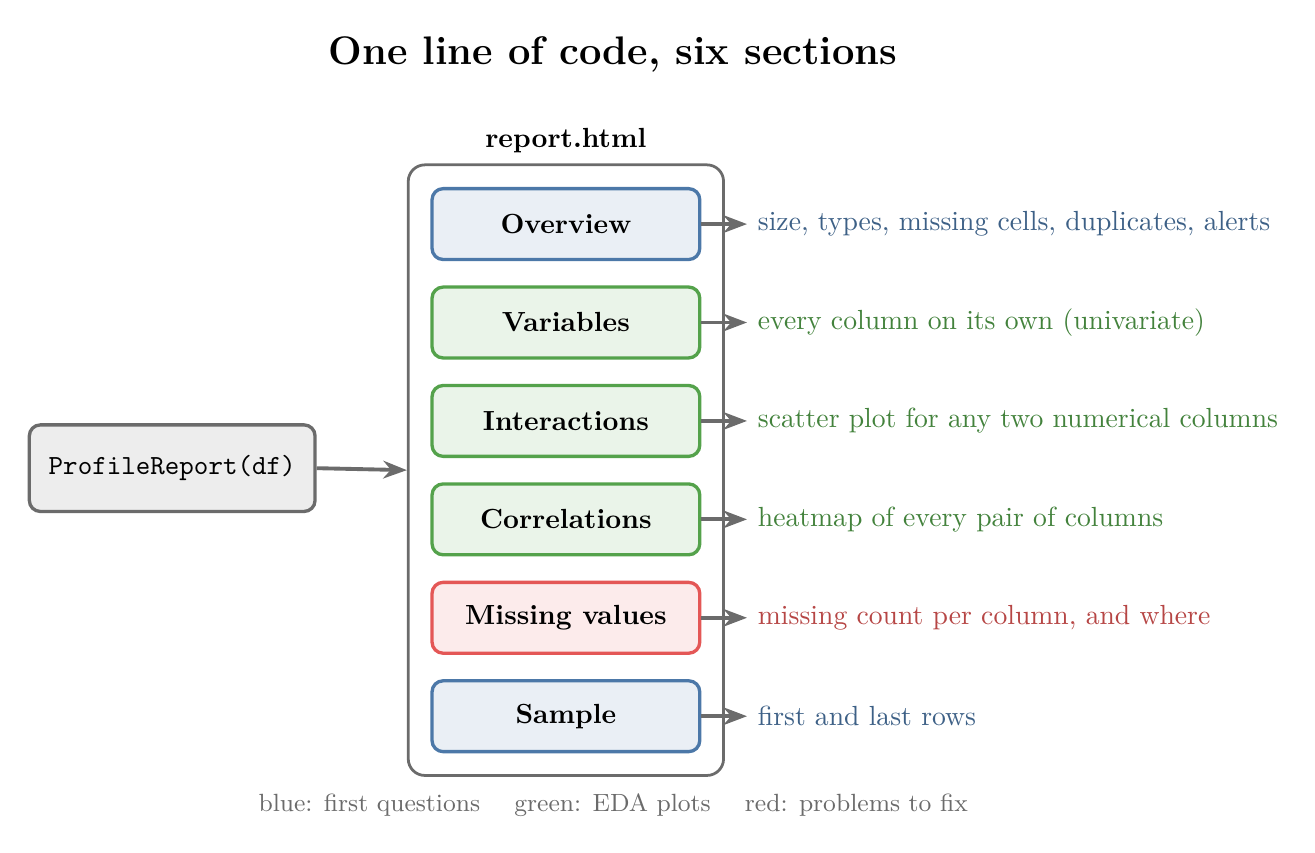
\begin{tikzpicture}
  \node[title] at (5.2,1.5) {One line of code, six sections};
  % the code that builds the report
  \node[box=cgrey, font=\ttfamily, minimum width=3.6cm] (code) at (-0.4,-3.75) {ProfileReport(df)};
  % the report page: a frame holding six section boxes
  \foreach \i/\s/\a/\col in {
      1/Overview/{size, types, missing cells, duplicates, alerts}/cblue,
      2/Variables/every column on its own (univariate)/cgreen,
      3/Interactions/scatter plot for any two numerical columns/cgreen,
      4/Correlations/heatmap of every pair of columns/cgreen,
      5/Missing values/{missing count per column, and where}/cred,
      6/Sample/first and last rows/cblue} {
    \node[box=\col, minimum width=3.4cm, minimum height=0.9cm, inner sep=4pt]
      (s\i) at (4.6,-1.25*\i+0.6) {\textbf{\s}};
    \node[anchor=west, text=\col!80!black] (a\i) at (6.9,-1.25*\i+0.6) {\a};
    \draw[arrow] (s\i.east) -- (a\i.west);
  }
  \node[draw=cgrey, rounded corners=6pt, line width=1pt, inner sep=8pt, fit=(s1)(s6),
        label={[font=\sffamily\bfseries]above:report.html}] (page) {};
  \draw[arrow] (code.east) -- (page.west);
  \node[note, anchor=north] at (5.2,-7.75) {blue: first questions \quad green: EDA plots \quad red: problems to fix};
\end{tikzpicture}
\end{document}
